\documentclass[border=3pt,varwidth]{standalone}
\usepackage{amsmath,amssymb}
\usepackage{tikz}
\usetikzlibrary{arrows.meta,calc,decorations.markings,patterns,positioning,angles,quotes}
\tikzset{
  >=Stealth,
  every node/.style={font=\normalsize},
  wire/.style={line width=0.9pt},
  thinwire/.style={line width=0.6pt},
  fieldline/.style={line width=0.6pt,-{Stealth[length=2.2mm]}},
  axis/.style={line width=0.7pt,-{Stealth[length=2.2mm]}},
  dashedwire/.style={line width=0.9pt,dash pattern=on 3pt off 2pt},
  resistor/.style={line width=0.9pt},
  chargepos/.style={circle,draw,line width=0.8pt,minimum size=5mm,inner sep=0pt},
  dotcharge/.style={circle,fill,inner sep=0pt,minimum size=2.4pt}
}
% Draw a resistor box centered at (x,y) with width w, height h, horizontal
\newcommand{\resbox}[4]{%
  % #1=x #2=y #3=halfwidth #4=label
  \draw[resistor] (#1-#3,#2-0.18) rectangle (#1+#3,#2+0.18);
  \ifx\\#4\\\else\node[above=2pt] at (#1,#2+0.18) {#4};\fi
}
% Battery symbol: long thin line (+) then short thick line (-), centered at (x,y)
\newcommand{\battery}[2]{%
  % #1=x #2=y ; long line left=+, short line right=- by default orientation
  \draw[wire] (#1-0.09,#2-0.32) -- (#1-0.09,#2+0.32);
  \draw[line width=2.6pt] (#1+0.09,#2-0.16) -- (#1+0.09,#2+0.16);
}

\begin{document}
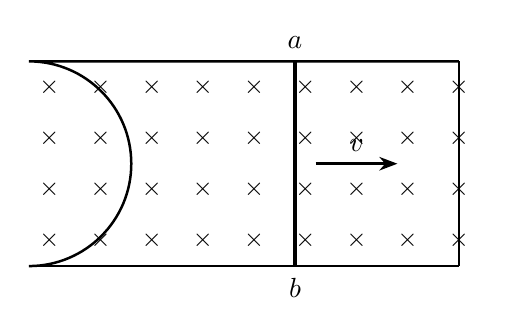
\begin{tikzpicture}[scale=1.3]
  % field region: grid of x marks (field into page)
  \foreach \x in {-2.1,-1.6,...,2.1} {
    \foreach \y in {-0.75,-0.25,0.25,0.75} {
      \node at (\x,\y) {\small $\times$};
    }
  }
  % loop: curved left end (bracket-style, like a C shape) and straight right end
  \draw[wire] (-2.3,-1.0) arc[start angle=-90,end angle=90,radius=1.0] -- (1.9,1.0);
  \draw[wire] (-2.3,-1.0) -- (1.9,-1.0);
  % right straight side of the loop
  \draw[wire] (1.9,1.0) -- (1.9,-1.0);
  % movable middle segment (rod) with points a (top) and b (bottom)
  \draw[wire,line width=1.2pt] (0.3,1.0) -- (0.3,-1.0);
  \node[above=1pt] at (0.3,1.0) {$a$};
  \node[below=1pt] at (0.3,-1.0) {$b$};
  % velocity arrow
  \draw[wire,-{Stealth[length=2.3mm]}] (0.5,0) -- (1.3,0);
  \node[above=1pt] at (0.9,0) {$v$};
\end{tikzpicture}
\end{document}
